\chapter{Cahier des besoins}

\section{Besoins fonctionnels}

\subsection{Besoin Utilisateurs}
\subsubsection{Créer des routes}
L'application doit permettre de créer des routes dans le réseau, c'est-à-dire de trouver un chemin allant du routeur d'entrée vers une autre cible. Il faudra donc modifier la table de routage du routeur d'entrée. Dans notre cas, la cible sera une adresse fictive et permettra un routage vers un trou noir pour contrer l'attaque.

\subsubsection{Supprimer des routes}
Puisqu'il permet la création, l'application devra permettre également la suppression des routes précédemment créées.

\subsubsection{Activer \& désactiver des routes}
Une fonction d'activation et de désactivation des routes existantes permettra de gérer les routes existantes sans les supprimer et donc sans avoir besoin de les recréer par la suite.

\subsubsection{Connexions \& Déconnexions}
Une page d'authentification permettra de restreindre l'accès de l'application et donc permettre que l'administrateur soit le seul à pouvoir se connecter.

\subsection{Interface utilisateur}
Pour permettre une gestion plus visuelle des différentes fonctions implémentées, une interface sera ajoutée. %geoff
 
\begin{figure}[H]
    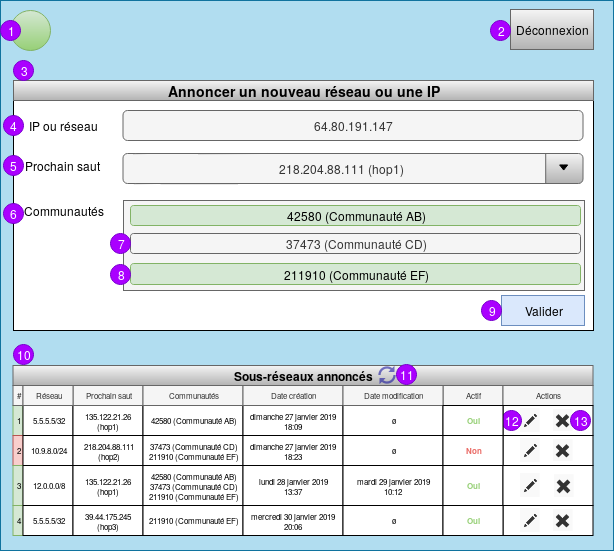
\includegraphics[width=\textwidth]{./medias/ui_interface.png}
    \caption{Prototype interface utilisateur}
    \label{fig:ui_interfaces}
\end{figure}


\subsection{Communication avec ExaBGP}
\noindent
La liste des commandes ExaBGP sont :
\begin{itemize}
    \item GET /api/exabgp/status (Donne le statu de exaBGP)
    \item GET /api/exabgp/command{?action} (Execute une commande exaBGP)
    \item GET /api/exabgp/commands (Donne la liste des commandes de exaBGP)
    \item GET /api/communities (Donne la liste des communities valides)
    \item GET /api/next\_hops (Donne la liste des next\_hops valides)

\end{itemize}

\subsubsection{Envoyer les routes}
Dès que l'utilisateur aura ajouté une route, il faut transmettre les informations à ExaBGP afin qu'il diffuse la route auprès des routeurs Cisco.

% Recevoir et utiliser l'information de l'autre groupe
%Même si nous ne savons pas clairement comme l'autre groupe va nous info

% recevoir des "sources" par l'api, considérées comme dangereuses
% utilises ces "sources" pour créer des routes
% utiliser ces routes pour rediriger ces "sources" dans le néant

\subsection{Définition de l'API REST}
Pour se baser sur l'architecture REST, nous organiserons nos URL en conséquence :
\begin{itemize}
    \item POST /api/routes (Créer une route)
    \item GET /api/routes/1 (Afficher la route 1)
    \item PUT /api/routes/1 (Remplacer la route 1)
    \item PATCH /api/routes/1 (Modifier la route 1)
    \item DELETE /api/routes/1 (Supprimer la route 1)
\end{itemize}

\subsubsection{Utilisation de HTTP 1.1}
Nous avons décidé d'utiliser HTTP 1.1 pour le développement de l'API. Bien que les performances soient accrues en HTTP 2, nous pensons que l'application sera assez légére pour ne pas avoir besoin de l'utiliser.

%\subsubsection{Client / Serveur}


\subsubsection{Stateless}
L’état de la session est entièrement conservé sur le client.

\subsubsection{Cache}
Nous mettrons en cache les communautés, les hops, la liste des routes existantes.

%\subsubsection{Interface uniforme}

%\subsubsection{Système en couches}

\subsubsection{Code à la demande}
\begin{itemize}
    \item Implémenter la possibilité d'exécuter des commandes lié à des fonctionnalité non relié à l'interface.
    \item L'interface de l'utilisateur sera implémentée en anglais. Une option pour traduire l'interface en français pourra être implémentée par la suite.
\end{itemize}

\begin{figure}[H]
    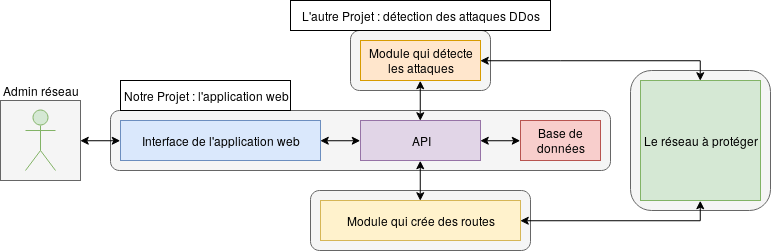
\includegraphics[width=\textwidth]{./medias/use_cases.png}
    \caption{Diagramme d'utilisation de l'application}
    \label{fig:use_cases}
\end{figure}

\newpage

\section{Besoins non fonctionnels}

\subsection{Coût}
Le développement de l'application ne devra entraîner aucun coût financier. C'est pourquoi, nous utiliseront que des logiciels open source sauf l'image CISCO qui nous sera fournie par le client .

\subsection{Performance}
% L'action décidée par l'administrateur doit pouvoir se faire rapidement
L'application devra être développée pour permettre une défense sur plusieurs attaques simultanées. % il faut chiffrer

\subsection{Authentifié}
L’application ne devra être utilisable que par l'administrateur. Donc, nous devons donc en place un service d'authentification pour permettre à l'administrateur seulement d'y avoir accès.

\subsection{Tester}
L'application sera testée sur un réseau virtuel avec au minimum deux routeur, une machine serveur et une machine cliente et attaquante. Les tests ne s'effectueront que sur le système d'exploitation debian.

\subsection{Fiabilité}
L'application devra être couverte par des tests pour vérifier que les différentes actions sur les routes sont bien implémentées et permettent donc bien de gérer un routage vers trou noir. C'est pourquoi, les tests doivent couvrir le code à hauteur de 80\%.

%\subsection{Pérennité ?}

%\subsection{Évolutivité ?}

%\subsection{Capacité ?}
